\documentclass[12pt]{exam}

\usepackage{amssymb}
\usepackage{mathtools}
\usepackage{algorithm}
\usepackage{float}  % Figure placement
\usepackage{minted}  % Code highlighting
\usepackage{tikz}  % Flow chart
\usepackage{lipsum}
\usepackage{xspace}
\usepackage{hyperref}
\usepackage{MnSymbol}
\usepackage{pgffor}
\usepackage{colortbl}
\usepackage{multirow}
\usepackage{array}


\hypersetup{
    colorlinks = true,
    linkcolor = blue,
    urlcolor  = blue,
    citecolor = blue,
    anchorcolor = blue
}

\newcommand{\hwheaderfooter}[3]{
\pagestyle{headandfoot}
\firstpageheadrule
\firstpageheader{#1}{#2}{#3}
\runningheader{#1}{#2}{#3}
\runningheadrule
\firstpagefooter{}{\thepage}{}
\runningfooter{}{\thepage}{}
}

\newcommand{\latex}{\LaTeX\xspace}

\newcommand{\stars}[1]{%
    \foreach \n in {1,...,#1}{%
        $\filledstar$%
    }%
}

\hwheaderfooter{Ching}{HW 9 Part 1}{CSCI 406}


\begin{document}
\begin{center}
    \fbox{\fbox{\parbox{\textwidth - 0.2 in}{\centering

                {Instructions: Please note that handwritten assignments \textbf{will not be graded}. Use the
                    provided \latex template to complete your homework. Please do not alter the order or spacing of
                    questions (keep each question on its own page). When you submit to Gradescope, you must mark
                    which page(s) correspond to each question. \textbf{You may not receive credit for unmarked
                        questions}. \\ When including graphical figures, we encourage the use of tools such as \href{https://dreampuf.github.io/GraphvizOnline/}{graphviz} or packages like \href{https://www.overleaf.com/learn/latex/TikZ_package}{tikz} for simple and complex figures. However, these may be handwritten only if they are neat and legible (as defined by the grader). }
            }}}
\end{center}

\textbf{List any collaborators (besides TAs or professors) here:}

\begin{questions}

    \question[15] [W10, \stars{1}] Edit Distance Traceback.

    Consider the following illustration of the edit distance between two gene sequences:
    \begin{center}
        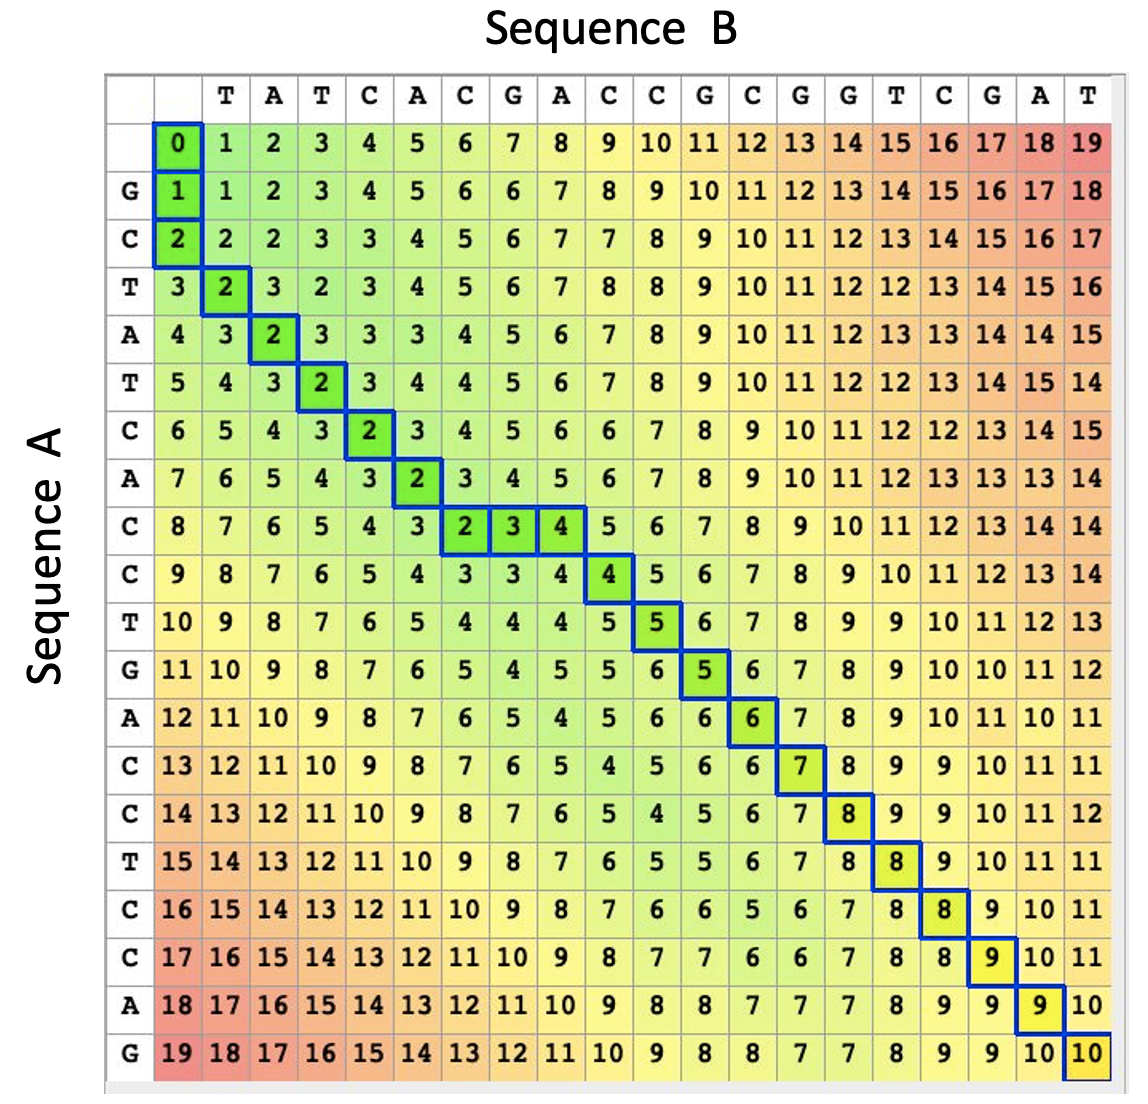
\includegraphics[width=0.5\textwidth]{genesequence.png}
    \end{center}

    Answer the following questions by filling in the boxes with ``insert", ``delete", ``match"
    or ``substitute" as appropriate:
    \begin{parts}
        \part[2] If the parent pointer of a cell points to the cell \textit{directly to the left}, then a(n) $\boxed{\text{ANSWER HERE}}$ in Sequence A occurred.
        \part[2] If the parent pointer of a cell points to the cell \textit{directly above}, then a(n) $\boxed{\text{ANSWER HERE}}$ in Sequence A occurred.
        \part[2] If the parent pointer of a cell points to the cell \textit{directly diagonal to the top-left}, and the values in the cells within the table are \textit{equal} then a(n) $\boxed{\text{ANSWER HERE}}$ occurred.
        \part[2] If the parent pointer of a cell points to the cell \textit{directly diagonal to the top-left}, and the values in the cells within the table are \textit{not equal} then a(n) $\boxed{\text{ANSWER HERE}}$ occurred.
        \part[7] Provide the edit trace for the example above in a format similar to the following:

        \begin{tabular}{ccccc} %\hline
            I               & A                 & G                 & O                 & -               \\ % \hline
            {\color{red} D} & {\color{green} M} & {\color{green} M} & {\color{green} M} & {\color{red} I} \\ %\hline
            -               & A                 & G                 & O                 & G               \\ % \hline
        \end{tabular}

    \end{parts}

    \clearpage

    \question[50] [W10, \stars{5}] A certain string processing language allows the programmer to break a string, into two pieces. It costs $n$ units of time to break a string, of $n$ characters into two
    pieces, since this involves copying the old string.

    You want to break a string, $A$, into $m$ pieces labeled $S_1, S_2, \dots, S_m$ with lengths of $l_1, l_2, \dots, l_m$, respectively. (Concatenating $S_1, S_2, \dots, S_{m}$ together would form $A$.)

    The order in which the breaks are made can affect the total amount of time used. For example, suppose you wish to break a 20-character string after characters 3, 8, and 10 (meaning $l_1=3, l_2=5, l_3=2, l_4=10$). If the breaks are made in left-right order, then the first break costs 20 units of time, the second break costs 17 units of time, and the third break costs 12 units of time, for a total of 49 units of time. If the breaks are made in right-left order, the first break costs 20 units of time, the second break costs 10 units of time, and the third break costs 8 units of time, for a total of only 38 units of time.

    Your task is to develop a dynamic programming algorithm that takes a list of piece lengths ($l_1, \dots, l_m$) and determines the cheapest break cost in $\mathcal{O}(n^3)$ time.

    \begin{parts}
        \part[10] Provide the optimal break cost for a string of length 20 and split pieces of lengths 3, 7, 6, 4.

        \part[5] What are the inputs to the \textbf{subproblem instance}?

        \part[5] Which subproblem instances are the \textbf{base cases}? What are their values?

        \part[15] Given your answers to the above questions, develop notation and write a \textit{formula} the \textbf{recurrence relation}.

        \part[5] How many \textbf{dimensions} will the dynamic programming table (used in bottom-up DP) have? What variables will each dimension of your table correspond to? What is the domain of each dimension?

        \part[10] What \textbf{iteration order} is required to compute the bottom-up DP table?

    \end{parts}

    % close the document
\end{questions}
\end{document}